\documentclass[12pt]{article}
\usepackage[utf8]{inputenc}
\usepackage[english]{babel}

\usepackage{minted}

\input{preamble.tex}


\title{\bfseries Project 1}
\author{Bryan Beus}
\date{\today}

\begin{document}

\maketitle

%%%%%%%%%%%%%%%%%%%%%%%%%%%%%%%%%%%%%%%%%%%%%%%%%%%%%%%%%%%%%%%%%%%%%%%
% DESIGN SECTION %%%%%%%%%%%%%%%%%%%%%%%%%%%%%%%%%%%%%%%%%%%%%%%%%%%%%%
%%%%%%%%%%%%%%%%%%%%%%%%%%%%%%%%%%%%%%%%%%%%%%%%%%%%%%%%%%%%%%%%%%%%%%%

\section{SQL Queries}

The following are the SQL queries used to obtain data from the tables.

I live in North Pole, AK, USA. The nearest city available in the \lstinline{city_data} table is Seattle. Temperatures for Seattle are available from \lstinline{1828} to \lstinline{2013}. Therefore, when extracting global data I excluded values for years prior to \lstinline{1828}.

\begin{minted}{sql}
SELECT year, city, avg_temp
FROM city_data
WHERE city='Seattle';
\end{minted}

\begin{minted}{sql}
SELECT *
FROM global_data
WHERE year>=1828 AND year<=2013;
\end{minted}

\pagebreak

\section{Organizing and Cleaning Data}

\subsection{Global Data}

Upon reviewing the CSV data in Google Sheets I found that the \lstinline{global_data} table provided clean data with no missing values.

I created a \lstinline{moving average} column and used the following command to create a moving average that considered \lstinline{10} years at a time.

\begin{minted}{sql}
=average(B2:B11)
\end{minted}

The following is a screenshot of the result.

\begin{center}
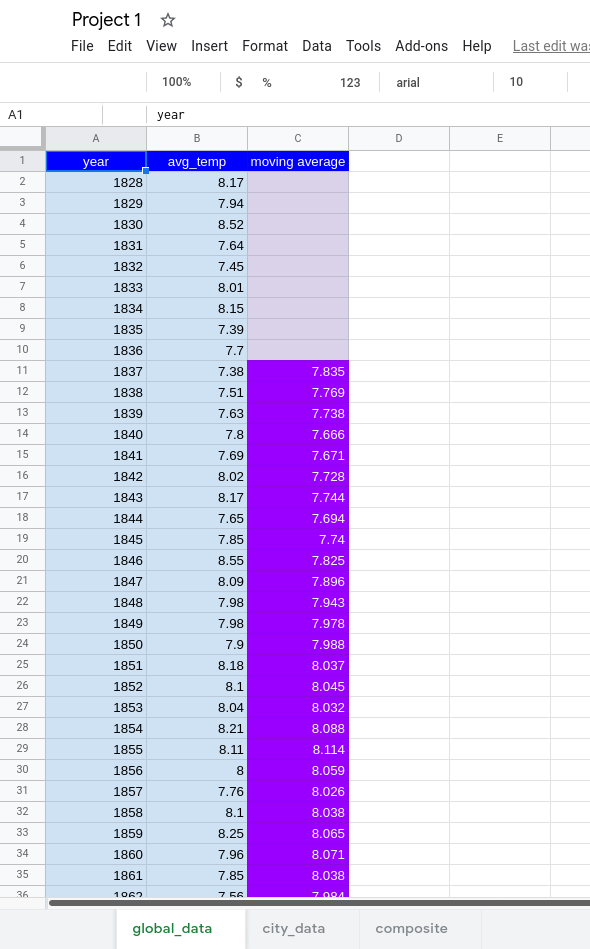
\includegraphics[width=0.5\textwidth]{global_data.png}
\end{center}

\pagebreak

\subsection{City Data}

The \lstinline{city_data} table values for Seattle lacked data for several dates.

To repair the missing values, I created an additional column called \lstinline{wrangled} that used the following spreadsheet command.

\begin{minted}{sql}
=IF(C2=0,D1,C2)
\end{minted}

I applied the above formula to all matching cells in this column. The result was that anywhere data was missing, the cell would automatically fill with the value that was inserted for the prior year.

Using the \lstinline{wrangled} column as the primary data column, I then performed the same steps as before to obtain a \lstinline{moving average} column of data, with the following result.

\begin{center}
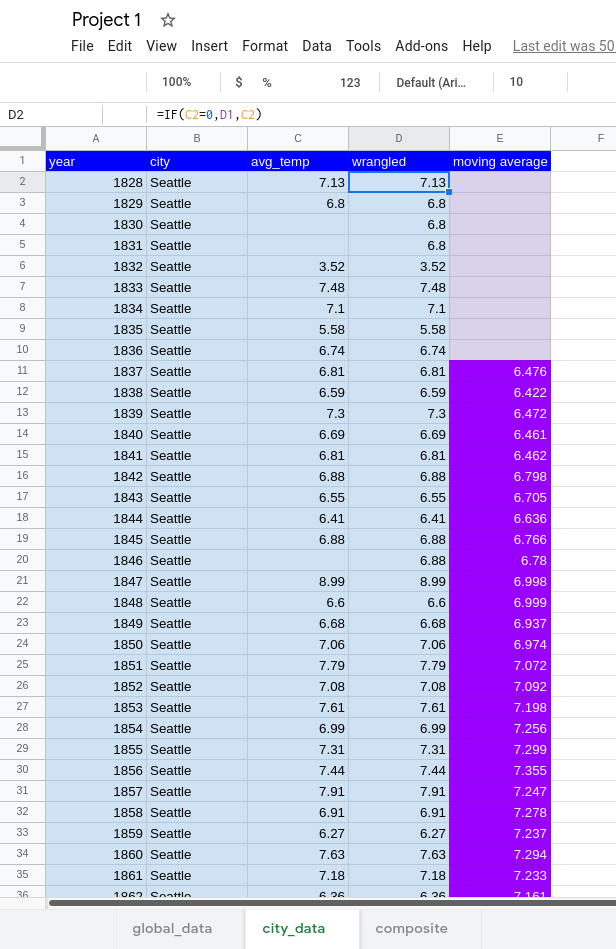
\includegraphics[width=0.5\textwidth]{city_data.png}
\end{center}

\pagebreak

\section{Analyzing the Data}

\subsection{Initial Compilation}

In a new spreadsheet I imported the \lstinline{year} column and the \lstinline{moving average} columns from both the global and city data.

Using the following commands I calculated the correlation coefficient.

\begin{minted}{sql}
=correl(B11:B187,C11:C187)
\end{minted}

To obtain the min, overall average, max, and standard deviation of the global temperatures, I executed the following spreadsheet commands.

\begin{minted}{sql}
=MIN(global_data!B2:B187)
=AVERAGE(global_data!B2:B187)
=MAX(global_data!B2:B187)
=STDEV(global_data!B2:B187)
\end{minted}

To obtain the Seattle equivalents, I performed the same commands on the matching data (not shown for brevity).

\pagebreak

\subsection{Line Graph}
Using the default Chart Tool in Google Sheets, I generated a line graph to display the data over the indicated years.

\begin{center}
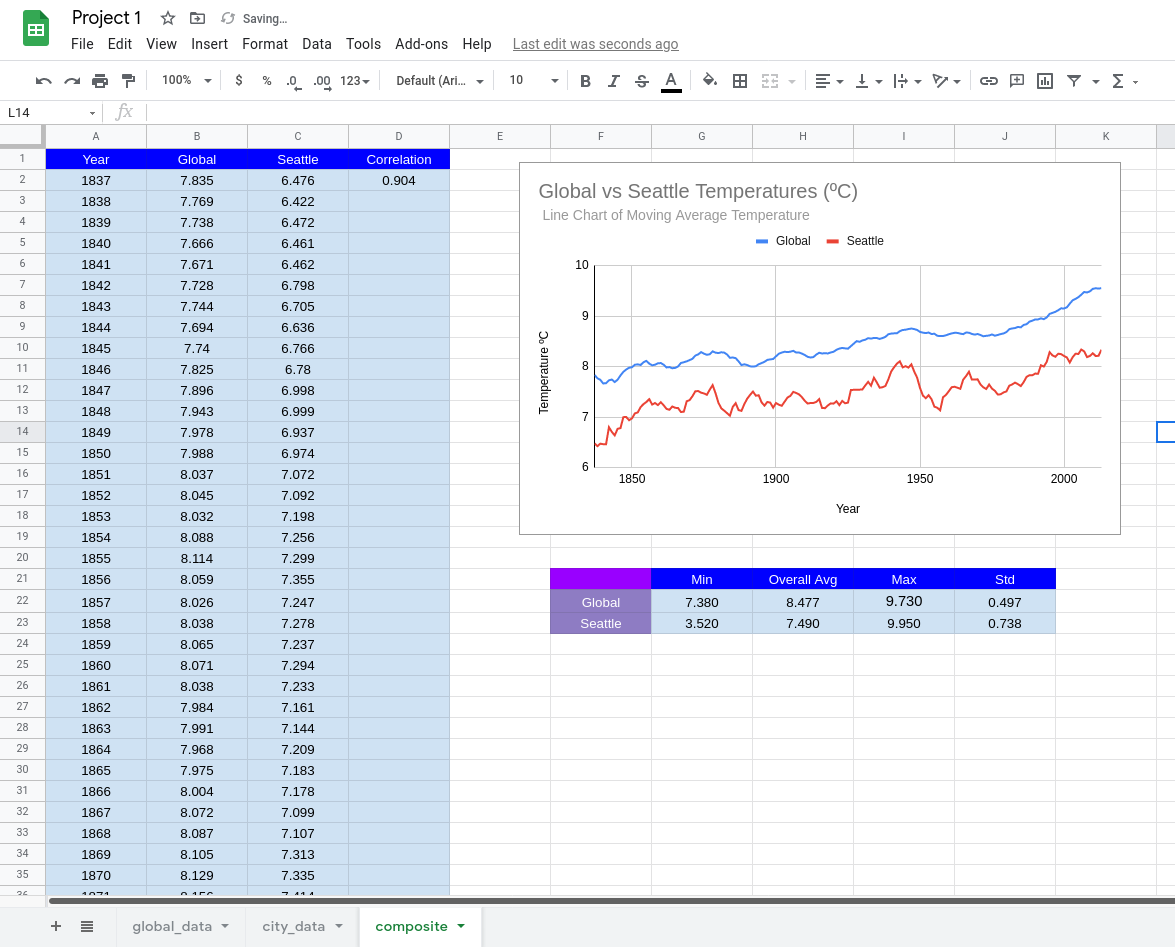
\includegraphics[width=0.5\textwidth]{composite.png}
\end{center}

\begin{center}
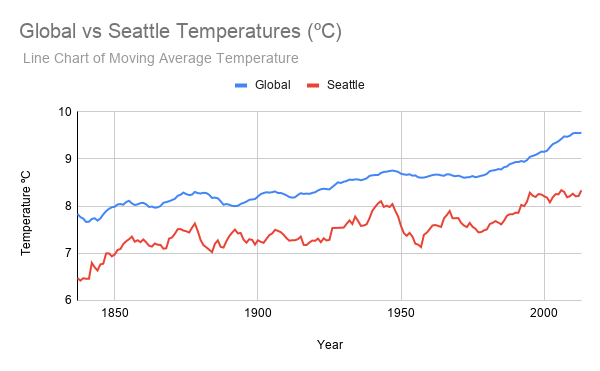
\includegraphics[width=0.8\textwidth]{line_graph.png}
\end{center}

\pagebreak

\subsection{Observations}

\begin{itemize}
    \item Seattle's overall average of 7.49 ºC is consistently cooler than the global average of 8.477 ºC. Perhaps this is due to Seattle's northern latitude.
    \item Seattle's standard deviation of 0.738 ºC is far higher than the global standard devision of 0.497 ºC. Perhaps this is due to Seattle's frequent inclement weather.
    \item A correlation coefficient of \lstinline{0.904} indicates that Seattle's temperature is highly correlated with the global temperature. Perhaps this is due to Seattle's location near the sea. This has the effect of bringing Seattle's temperature into alignment with a far greater surface area due to the manner in which the sea currents conduct temperatures from abroad.
    \item The temperature does seem to be increasing over the past approximately two hundred years. Seattle's temperature begins at approximately 6.5 ºC, rises consistently for the given time span, and ends at approximately 8.2 ºC. The global temperature begins at approximately 7.8 ºC, rises consistently for the given time span, and ends at approximately 9.6 ºC. The cause for this rise in temperature is not clear and is hotly debated, sometimes out of a sincere desire to forestall global catastrophe, and sometimes due to political and corporate agendas.
\end{itemize}


\iffalse

%%%%%%%%%%%%%%%%%%%%%%%%%%%%%%%%%%%%%%%%%%%%%%%%%%%%%%%%%%%%%%%%%%%%%%%
% LINKS SECTION %%%%%%%%%%%%%%%%%%%%%%%%%%%%%%%%%%%%%%%%%%%%%%%%%%%%%%%
%%%%%%%%%%%%%%%%%%%%%%%%%%%%%%%%%%%%%%%%%%%%%%%%%%%%%%%%%%%%%%%%%%%%%%%

\begin{itemize}
\item Repository Link:
% This is where you will put a link to your GitHub project
\url{https://www.github.com/yourusername/cs202/}

% This is where you will put a link to your GitHub project commits
\item Git Commits:
\url{https://www.github.com/yourusername/cs202/commits}

% PLEASE NOTE THE AMOUNT OF TIME THIS HOMEWORK TOOK

\item This homework took approximately XX hours to complete.
\end{itemize}



%%%%%%%%%%%%%%%%%%%%%%%%%%%%%%%%%%%%%%%%%%%%%%%%%%%%%%%%%%%%%%%%%%%%%%%
% DESIGN SECTION %%%%%%%%%%%%%%%%%%%%%%%%%%%%%%%%%%%%%%%%%%%%%%%%%%%%%%
%%%%%%%%%%%%%%%%%%%%%%%%%%%%%%%%%%%%%%%%%%%%%%%%%%%%%%%%%%%%%%%%%%%%%%%

\section{Design}

In this section, you will write a paragraph in about 100 words about the design you took for this program. You are encouraged to also write about the design of your other programs. You are encouraged to make one page designs for your programs as well.




%%%%%%%%%%%%%%%%%%%%%%%%%%%%%%%%%%%%%%%%%%%%%%%%%%%%%%%%%%%%%%%%%%%%%%%
% POST MORTEM SECTION %%%%%%%%%%%%%%%%%%%%%%%%%%%%%%%%%%%%%%%%%%%%%%%%%
%%%%%%%%%%%%%%%%%%%%%%%%%%%%%%%%%%%%%%%%%%%%%%%%%%%%%%%%%%%%%%%%%%%%%%%

\section{Post Mortem}

In this section, you will write a paragraph in about 100 words about what went right and what went wrong for this assignment. What lessons were learned or best practices identified?




%%%%%%%%%%%%%%%%%%%%%%%%%%%%%%%%%%%%%%%%%%%%%%%%%%%%%%%%%%%%%%%%%%%%%%%
% QUESTION ANSWER SECTION %%%%%%%%%%%%%%%%%%%%%%%%%%%%%%%%%%%%%%%%%%%%%
%%%%%%%%%%%%%%%%%%%%%%%%%%%%%%%%%%%%%%%%%%%%%%%%%%%%%%%%%%%%%%%%%%%%%%%

\section{Answers to Questions}

In this section, you will write the answers to the questions in the homework assignment.

\begin{enumerate}
    \item Answer to question 1 \ldots
    \item Answer to question 2 \ldots
    \item \ldots
\end{enumerate}




%%%%%%%%%%%%%%%%%%%%%%%%%%%%%%%%%%%%%%%%%%%%%%%%%%%%%%%%%%%%%%%%%%%%%%%
% PROGRAM 1 SECTION %%%%%%%%%%%%%%%%%%%%%%%%%%%%%%%%%%%%%%%%%%%%%%%%%%%
%%%%%%%%%%%%%%%%%%%%%%%%%%%%%%%%%%%%%%%%%%%%%%%%%%%%%%%%%%%%%%%%%%%%%%%

\section{Program 1}

%%%%%%%%%%%%%%%%%%%%%%%%%%%%%%%%%%%%%%%%%%%%%%%%%%%%%%%%%%%%
%% SAMPLE OUTPUT / SCREENSHOT %%%%%%%%%%%%%%%%%%%%%%%%%%%%%%
%%%%%%%%%%%%%%%%%%%%%%%%%%%%%%%%%%%%%%%%%%%%%%%%%%%%%%%%%%%%
\subsection{Sample Output/Screenshot}

% We are going to color the output BLUE, and then set it back to BLACK
% The lstlisting environment documentation may be found
% https://en.wikibooks.org/wiki/LaTeX/Source_Code_Listings
% http://tug.ctan.org/macros/latex/contrib/listings/listings.pdf
\lstset{language=, caption=Sample Program Output, label=lst:output}
\color{blue}
\begin{lstlisting}
Hello, world
PUT YOUR OUTPUT HERE
\end{lstlisting}
\color{black}

Or you can put a screenshot:

% Or a screenshot
\begin{center}
\includegraphics[width=0.5\textwidth]{screenshot.png}
\end{center}

%%%%%%%%%%%%%%%%%%%%%%%%%%%%%%%%%%%%%%%%%%%%%%%%%%%%%%%%%%%%
%% GIT COMMIT MESSAGES %%%%%%%%%%%%%%%%%%%%%%%%%%%%%%%%%%%%%
%%%%%%%%%%%%%%%%%%%%%%%%%%%%%%%%%%%%%%%%%%%%%%%%%%%%%%%%%%%%
\subsection{Git Commit Messages}

\begin{centering}
\begin{tabularx}{\linewidth}{c X}
\thead{Date} & \thead{Message} \\
\hline
2019-11-07 & \text{fix crash where maxhistorylines was 0 in hflog} \\
2019-11-07 & \text{Add pitch() method to TImage} \\
\hline
\end{tabularx}
\end{centering}


%%%%%%%%%%%%%%%%%%%%%%%%%%%%%%%%%%%%%%%%%%%%%%%%%%%%%%%%%%%%
%% SOURCE CODE %%%%%%%%%%%%%%%%%%%%%%%%%%%%%%%%%%%%%%%%%%%%%
%%%%%%%%%%%%%%%%%%%%%%%%%%%%%%%%%%%%%%%%%%%%%%%%%%%%%%%%%%%%
\subsection{Source Code}

% You could also \inputminted{c++}{myfile.cpp}
% or just put it here in the minted environment
\begin{minted}{c++}
#include <iostream>
#include "triangle.hpp"

using std::cout;
using std::endl;

int main(int argc, char **argv)
{
    cout << "Hello, World\n";
    Triangle t;
    t.print();
    return 0;
}
\end{minted}

\subsection{Triangle Header}

\inputminted{c++}{triangle.hpp}

\subsection{Triangle Source}

\inputminted{c++}{triangle.cpp}




%%%%%%%%%%%%%%%%%%%%%%%%%%%%%%%%%%%%%%%%%%%%%%%%%%%%%%%%%%%%%%%%%%%%%%%
% PROGRAM 2 SECTION %%%%%%%%%%%%%%%%%%%%%%%%%%%%%%%%%%%%%%%%%%%%%%%%%%%
%%%%%%%%%%%%%%%%%%%%%%%%%%%%%%%%%%%%%%%%%%%%%%%%%%%%%%%%%%%%%%%%%%%%%%%

\section{Program 2}


\subsection{Sample Output / Screenshot}
% \begin{center}
% \includegraphics[width=0.5\textwidth]{screenshot.png}
% \end{center}


\subsection{Git Commit Messages}

\begin{centering}
\begin{tabularx}{\linewidth}{c X}
\thead{Date} & \thead{Message} \\
\hline
2019-11-07 & fix crash where maxhistorylines was 0 in hflog \\
2019-11-07 & Add pitch() method to TImage \\
\hline
\end{tabularx}
\end{centering}


\subsection{Source Code}
% \inputminted{c++}{main.cpp}


%\subsection{File.hpp}
% \inputminted{c++}{File.hpp}


%\subsection{File.cpp}
% \inputminted{c++}{File.cpp}




%%%%%%%%%%%%%%%%%%%%%%%%%%%%%%%%%%%%%%%%%%%%%%%%%%%%%%%%%%%%%%%%%%%%%%%
% PROGRAM 3 SECTION %%%%%%%%%%%%%%%%%%%%%%%%%%%%%%%%%%%%%%%%%%%%%%%%%%%
%%%%%%%%%%%%%%%%%%%%%%%%%%%%%%%%%%%%%%%%%%%%%%%%%%%%%%%%%%%%%%%%%%%%%%%

\section{Program 3}

\subsection{Sample Output / Screenshot}
% \begin{center}
% \includegraphics[width=0.5\textwidth]{screenshot.png}
% \end{center}

\subsection{GitHub Commit Messages}

\begin{centering}
\begin{tabularx}{\linewidth}{c X}
\thead{Date} & \thead{Message} \\
\hline
2019-11-07 & \text{fix crash where maxhistorylines was 0 in hflog} \\
2019-11-07 & \text{Add pitch() method to TImage} \\
\hline
\end{tabularx}
\end{centering}

\subsection{Source Code}
% \inputminted{c++}{main.cpp}


%\subsection{File.hpp}
% \inputminted{c++}{File.hpp}


%\subsection{File.cpp}
% \inputminted{c++}{File.cpp}

\fi

\end{document}

